\documentclass[11pt,a4paper]{article}
\usepackage[utf8]{inputenc}
\usepackage[T1]{fontenc}
\usepackage[french]{babel}
\usepackage{lmodern}
\usepackage[margin=2.3cm]{geometry}
\usepackage{amsmath,amssymb,amsthm,mathtools,bm}
\usepackage{graphicx}
\usepackage{booktabs}
\usepackage{siunitx}
\sisetup{locale=FR}
\usepackage{xcolor}
\usepackage{listings}
\usepackage{caption}
\usepackage{float}
\usepackage[colorlinks=true,linkcolor=blue!50!black,citecolor=blue!50!black,urlcolor=blue!50!black]{hyperref}

\graphicspath{{../results/figures/}}
\newcommand{\TabSpace}{%
\begin{tabular}{c r r c c c c}\toprule
Élément & $N$ & ddl & $\|e\|_{L^2}$ & ordre & $|e|_{H^1}$ & ordre \\ \midrule
$\mathbb{P}_1$ & 4 & 25 & $\num{1.16}\cdot 10^{-1}$ & -- & $\num{1.26}\cdot 10^{0}$ & -- \\
 & 8 & 81 & $\num{3.09}\cdot 10^{-2}$ & \num{1.91} & $\num{6.48}\cdot 10^{-1}$ & \num{0.96} \\
 & 16 & 289 & $\num{7.85}\cdot 10^{-3}$ & \num{1.98} & $\num{3.26}\cdot 10^{-1}$ & \num{0.99} \\
 & 32 & 1\,089 & $\num{1.97}\cdot 10^{-3}$ & \num{1.99} & $\num{1.63}\cdot 10^{-1}$ & \num{1.00} \\
 & 64 & 4\,225 & $\num{4.93}\cdot 10^{-4}$ & \num{2.00} & $\num{8.18}\cdot 10^{-2}$ & \num{1.00} \\
\midrule
$\mathbb{P}_2$ & 4 & 81 & $\num{5.64}\cdot 10^{-3}$ & -- & $\num{1.94}\cdot 10^{-1}$ & -- \\
 & 8 & 289 & $\num{7.13}\cdot 10^{-4}$ & \num{2.98} & $\num{5.01}\cdot 10^{-2}$ & \num{1.96} \\
 & 16 & 1\,089 & $\num{8.93}\cdot 10^{-5}$ & \num{3.00} & $\num{1.26}\cdot 10^{-2}$ & \num{1.99} \\
 & 32 & 4\,225 & $\num{1.12}\cdot 10^{-5}$ & \num{3.00} & $\num{3.16}\cdot 10^{-3}$ & \num{2.00} \\
 & 64 & 16\,641 & $\num{1.40}\cdot 10^{-6}$ & \num{3.00} & $\num{7.92}\cdot 10^{-4}$ & \num{2.00} \\
\midrule
$\mathbb{P}_3$ & 4 & 169 & $\num{4.17}\cdot 10^{-4}$ & -- & $\num{1.99}\cdot 10^{-2}$ & -- \\
 & 8 & 625 & $\num{2.40}\cdot 10^{-5}$ & \num{4.12} & $\num{2.48}\cdot 10^{-3}$ & \num{3.00} \\
 & 16 & 2\,401 & $\num{1.44}\cdot 10^{-6}$ & \num{4.06} & $\num{3.09}\cdot 10^{-4}$ & \num{3.01} \\
 & 32 & 9\,409 & $\num{8.80}\cdot 10^{-8}$ & \num{4.03} & $\num{3.85}\cdot 10^{-5}$ & \num{3.00} \\
 & 64 & 37\,249 & $\num{5.45}\cdot 10^{-9}$ & \num{4.01} & $\num{4.81}\cdot 10^{-6}$ & \num{3.00} \\
\bottomrule\end{tabular}}
\newcommand{\TabTime}{%
\begin{tabular}{c r c c c c}\toprule
 & & \multicolumn{2}{c}{Euler implicite ($\theta=1$)} & \multicolumn{2}{c}{Crank--Nicolson ($\theta=\frac12$)} \\
\cmidrule(lr){3-4}\cmidrule(lr){5-6}
$\Delta t$ & pas & $\|e(T)\|_{L^2}$ & ordre & $\|e(T)\|_{L^2}$ & ordre \\ \midrule
$\num{0.2}$ & 5 & $\num{2.78}\cdot 10^{-3}$ & -- & $\num{8.75}\cdot 10^{-5}$ & -- \\
$\num{0.1}$ & 10 & $\num{1.34}\cdot 10^{-3}$ & \num{1.05} & $\num{2.15}\cdot 10^{-5}$ & \num{2.02} \\
$\num{0.05}$ & 20 & $\num{6.59}\cdot 10^{-4}$ & \num{1.03} & $\num{5.39}\cdot 10^{-6}$ & \num{2.00} \\
$\num{0.025}$ & 40 & $\num{3.26}\cdot 10^{-4}$ & \num{1.01} & $\num{1.35}\cdot 10^{-6}$ & \num{2.00} \\
$\num{0.0125}$ & 80 & $\num{1.62}\cdot 10^{-4}$ & \num{1.01} & $\num{3.37}\cdot 10^{-7}$ & \num{2.00} \\
$\num{0.00625}$ & 160 & $\num{8.10}\cdot 10^{-5}$ & \num{1.00} & $\num{8.44}\cdot 10^{-8}$ & \num{2.00} \\
\bottomrule\end{tabular}}
\newcommand{\LamMin}{\num{19.930}}
\newcommand{\LamMinExact}{\num{19.739}}
\newcommand{\LamMax}{\num{6466.9}}
\newcommand{\DtC}{\num{3.093}\cdot 10^{-4}}
\newcommand{\RatioStable}{\num{0.949}}
\newcommand{\RatioUnstable}{\num{1.050}}
\newcommand{\NormStable}{\num{1.102}}
\newcommand{\NormUnstable}{\num{2.0}\cdot 10^{29}}
\newcommand{\CNmin}{\num{-0.525}}
\newcommand{\CNmax}{\num{0.702}}
\newcommand{\BEmin}{\num{0.000}}
\newcommand{\BEmax}{\num{0.475}}
\newcommand{\REFmax}{\num{0.307}}
\newcommand{\LaserTmax}{\num{601.7}}
\newcommand{\LaserProbeA}{\num{596.9}}
\newcommand{\LaserProbeB}{\num{285.0}}
\newcommand{\LaserProbeC}{\num{163.9}}
\newcommand{\LaserEin}{\num{3005.00}}
\newcommand{\LaserEout}{\num{350.3}}
\newcommand{\LaserEstored}{\num{2654.7}}
\newcommand{\LaserLossPct}{\num{11.7}}
\newcommand{\LaserBalance}{\num{3.7}\cdot 10^{-13}}
\newcommand{\LaserNdofs}{20\,301}
\newcommand{\LaserWall}{\num{18}}
\newcommand{\TabLaserConv}{%
\begin{tabular}{l r r r c c c}\toprule
Cas & $h$ (mm) & $\Delta t$ (s) & ddl & $\max T$ (°C) & écart / réf. & $T_{\text{sonde }0}$ (°C) \\ \midrule
maillage $100\times50$ & \num{1} & \num{0.05} & 5\,151 & \num{600.52} & \num{-1.52} & \num{595.73} \\
maillage $200\times100$ & \num{0.5} & \num{0.05} & 20\,301 & \num{601.73} & \num{-0.31} & \num{596.95} \\
maillage $400\times200$ & \num{0.25} & \num{0.05} & 80\,601 & \num{602.04} & \num{+0.00} & \num{597.26} \\
\midrule
pas $\Delta t = \num{0.1}$ & \num{0.5} & \num{0.1} & 20\,301 & \num{601.68} & \num{-0.36} & \num{596.09} \\
maillage $200\times100$ & \num{0.5} & \num{0.05} & 20\,301 & \num{601.73} & \num{-0.31} & \num{596.95} \\
pas $\Delta t = \num{0.025}$ & \num{0.5} & \num{0.025} & 20\,301 & \num{601.74} & \num{-0.30} & \num{596.96} \\
\bottomrule\end{tabular}}
\newcommand{\TabMPI}{%
\begin{tabular}{c l c r c c}\toprule
Processus MPI & Solveur & it. KSP / pas & temps (s) & accélération & $\max T$ (°C) \\ \midrule
1 & LU (MUMPS) & \num{1.0} & \num{74.5} & \num{1.00} & \num{602.038726} \\
2 & LU (MUMPS) & \num{1.0} & \num{66.5} & \num{1.12} & \num{602.038726} \\
1 & CG + BoomerAMG & \num{5.0} & \num{90.1} & \num{1.00} & \num{602.038726} \\
2 & CG + BoomerAMG & \num{5.9} & \num{73.6} & \num{1.22} & \num{602.038726} \\
\bottomrule\end{tabular}}
\newcommand{\NdofsMPI}{80\,601}
\newcommand{\ScalCPU}{12th Gen Intel\textsuperscript{\textregistered} Core\texttrademark{} i5-12450HX}
\newcommand{\ScalNdofs}{180\,901}
\newcommand{\ScalReps}{\num{3}}
\newcommand{\ScalTmaxSpread}{\num{3.1}\cdot 10^{-9}}
\newcommand{\ScalMaxSpread}{\num{0.6}}
\newcommand{\ScalSOne}{\num{1.00}}
\newcommand{\ScalEOne}{\num{100}}
\newcommand{\ScalTOne}{\num{176.7}}
\newcommand{\ScalSTwo}{\num{1.86}}
\newcommand{\ScalETwo}{\num{93}}
\newcommand{\ScalTTwo}{\num{94.8}}
\newcommand{\ScalSFour}{\num{3.12}}
\newcommand{\ScalEFour}{\num{78}}
\newcommand{\ScalTFour}{\num{56.6}}
\newcommand{\ScalSEight}{\num{2.46}}
\newcommand{\ScalEEight}{\num{31}}
\newcommand{\ScalTEight}{\num{71.9}}
\newcommand{\TabScaling}{%
\begin{tabular}{c r c c c c}\toprule
Processus & temps médian (s) & dispersion & it.\ CG / pas & accélération $S(p)$ & efficacité $E(p)$ \\ \midrule
1 & \num{176.7} & \num{0.6}~\% & \num{5.97} & \num{1.00} & \num{100}~\% \\
2 & \num{94.8} & \num{0.0}~\% & \num{6.00} & \num{1.86} & \num{93}~\% \\
4 & \num{56.6} & \num{0.5}~\% & \num{6.00} & \num{3.12} & \num{78}~\% \\
8 & \num{71.9} & \num{0.5}~\% & \num{6.81} & \num{2.46} & \num{31}~\% \\
\bottomrule\end{tabular}}


\newcommand{\R}{\mathbb{R}}
\newcommand{\dd}{\,\mathrm{d}}
\newcommand{\Pk}{\mathbb{P}_k}
\DeclareMathOperator{\divg}{div}
\newtheorem{proposition}{Proposition}

\lstdefinestyle{py}{
  language=Python, basicstyle=\ttfamily\footnotesize, keywordstyle=\color{blue!60!black}\bfseries,
  commentstyle=\color{green!40!black}\itshape, stringstyle=\color{red!60!black},
  frame=single, rulecolor=\color{gray!50}, backgroundcolor=\color{gray!5},
  breaklines=true, showstringspaces=false, columns=fullflexible, xleftmargin=1em, framexleftmargin=1em,
  literate={é}{{\'e}}1 {è}{{\`e}}1 {à}{{\`a}}1 {ê}{{\^e}}1
}
\lstset{style=py}

\title{\textbf{Équation de la chaleur instationnaire par éléments finis avec FEniCSx}\\[0.4em]
\large Vérification, analyse de stabilité et application à une source laser mobile}
\author{Ayoub Gounnou}
\date{14 novembre 2026}

\begin{document}
\maketitle

\begin{abstract}
On résout l'équation de la chaleur instationnaire par la méthode des éléments finis de Lagrange
$\mathbb{P}_1$--$\mathbb{P}_3$ avec DOLFINx~0.11 (FEniCSx), couplée à un $\theta$-schéma en temps
(Euler implicite, Crank--Nicolson, Euler explicite). Le code est vérifié par la méthode des solutions
manufacturées : les ordres de convergence théoriques $\mathcal{O}(h^{k+1})$ en norme $L^2$,
$\mathcal{O}(h^{k})$ en semi-norme $H^1$, $\mathcal{O}(\Delta t)$ pour Euler implicite et
$\mathcal{O}(\Delta t^2)$ pour Crank--Nicolson sont retrouvés à deux décimales près. La limite de
stabilité d'Euler explicite, $\Delta t_c = 2/\lambda_{\max}$, est calculée par un problème aux valeurs
propres généralisé puis confirmée numériquement, et le défaut de L-stabilité de Crank--Nicolson est mis
en évidence sur une donnée initiale discontinue. Le solveur est enfin appliqué au chauffage d'une plaque
d'acier par un laser mobile, avec pertes convectives : la conservation discrète de l'énergie est vérifiée
à la précision machine ($\LaserBalance$), l'indépendance au maillage et au pas de temps est établie, et le
calcul est exécuté en parallèle MPI avec des résultats identiques au calcul séquentiel. Une étude de
scalabilité forte sur un CPU hybride de portable donne une accélération de $\ScalSFour$ sur 4 processus,
puis une dégradation à 8, que l'on relie au déséquilibre entre cœurs performants et cœurs efficaces.
\end{abstract}

\tableofcontents
\newpage

%=====================================================================
\section{Introduction}
%=====================================================================
L'équation de la chaleur est le prototype des problèmes paraboliques. Elle intervient en thermique
(soudage, traitement de surface, refroidissement de composants électroniques), mais aussi comme
sous-problème de nombreux solveurs multiphysiques : étape de diffusion des schémas de projection en
mécanique des fluides, régularisation, problèmes de diffusion--réaction.

Les objectifs de ce projet sont :
\begin{enumerate}
  \item formuler le problème variationnel et sa discrétisation espace--temps ;
  \item implémenter un solveur générique et réutilisable avec FEniCSx (DOLFINx, UFL, PETSc) ;
  \item \emph{vérifier} le code, c'est-à-dire montrer qu'il résout correctement les équations, par des
        études de convergence quantitatives ;
  \item étudier la stabilité des schémas en temps et confronter la théorie aux calculs ;
  \item traiter un cas applicatif réaliste (source laser mobile) avec des contrôles de qualité :
        bilan d'énergie, indépendance au maillage, exécution parallèle.
\end{enumerate}

Tout le code, les données et les figures sont reproductibles par un seul script
(\texttt{run\_all.sh}, annexe~\ref{app:repro}). Aucun chiffre de ce rapport n'est recopié à la main :
les tableaux sont générés automatiquement à partir des fichiers de résultats.

%=====================================================================
\section{Modèle mathématique}
%=====================================================================
\subsection{Problème fort}
Soit $\Omega\subset\R^2$ un domaine borné de frontière $\partial\Omega = \Gamma_D \cup \Gamma_R \cup \Gamma_N$
et $T_f>0$. On cherche $u(\bm{x},t)$ telle que
\begin{equation}\label{eq:strong}
\left\{
\begin{aligned}
  \frac{\partial u}{\partial t} - \divg(\kappa \nabla u) + \beta\,(u - u_a) &= f
      && \text{dans } \Omega \times (0,T_f], \\
  u &= g && \text{sur } \Gamma_D \times (0,T_f], \\
  -\kappa \nabla u \cdot \bm{n} &= h_c\,(u - u_a) && \text{sur } \Gamma_R \times (0,T_f], \\
  \kappa \nabla u \cdot \bm{n} &= 0 && \text{sur } \Gamma_N \times (0,T_f], \\
  u(\cdot,0) &= u_0 && \text{dans } \Omega,
\end{aligned}
\right.
\end{equation}
où $\kappa>0$ est la diffusivité, $\beta\ge 0$ un coefficient d'échange volumique (utilisé en
section~\ref{sec:laser} pour la convection des faces d'une plaque mince), $h_c\ge0$ un coefficient de
Robin, $u_a$ la température ambiante et $f$ un terme source.

\subsection{Formulation variationnelle}
On note $V_g = \{v\in H^1(\Omega) : v = g \text{ sur } \Gamma_D\}$ et $V_0$ l'espace homogène
correspondant. On multiplie \eqref{eq:strong} par $v\in V_0$, on intègre sur $\Omega$ et on applique la
formule de Green :
\[
  -\int_\Omega \divg(\kappa\nabla u)\, v \dd x
  = \int_\Omega \kappa \nabla u\cdot\nabla v \dd x - \int_{\partial\Omega} \kappa \nabla u\cdot\bm{n}\, v \dd s .
\]
Le terme de bord s'annule sur $\Gamma_D$ (car $v=0$) et sur $\Gamma_N$, et vaut
$-\int_{\Gamma_R} h_c(u-u_a)v\dd s$ sur $\Gamma_R$. Le problème faible s'écrit donc : pour presque
tout $t$, trouver $u(t)\in V_g$ tel que
\begin{equation}\label{eq:weak}
  \left(\partial_t u, v\right) + a(u,v) = \ell(t; v) \qquad \forall v \in V_0,
\end{equation}
avec
\begin{align*}
  a(u,v) &= \int_\Omega \kappa\nabla u\cdot\nabla v \dd x + \int_\Omega \beta\, u\, v\dd x
            + \int_{\Gamma_R} h_c\, u\, v \dd s, \\
  \ell(t;v) &= \int_\Omega f\, v\dd x + \int_\Omega \beta\, u_a\, v \dd x + \int_{\Gamma_R} h_c\, u_a\, v\dd s .
\end{align*}
La forme $a$ est continue et coercive sur $V_0$ (dès que $|\Gamma_D|>0$, ou que $\beta>0$ ou
$h_c>0$ sur une partie de mesure non nulle), ce qui assure le caractère bien posé de \eqref{eq:weak}
(théorème de Lions).

\subsection{Bilan d'énergie}\label{sec:energy}
Dans le cas sans condition de Dirichlet ($\Gamma_D=\emptyset$), la fonction $v\equiv 1$ est admissible
et \eqref{eq:weak} donne le bilan global
\begin{equation}\label{eq:energy}
  \frac{\mathrm{d}}{\mathrm{d}t}\int_\Omega u \dd x
  = \underbrace{\int_\Omega f \dd x}_{\text{apport}}
  - \underbrace{\int_\Omega \beta(u-u_a)\dd x - \int_{\Gamma_R} h_c(u-u_a)\dd s}_{\text{pertes}} .
\end{equation}
Comme $1$ appartient aussi à l'espace discret, cette identité est satisfaite \emph{exactement} par le
schéma discret (au moyennage en $\theta$ près, voir section~\ref{sec:theta}). C'est un test de non-régression
très sévère, utilisé en section~\ref{sec:laser}.

%=====================================================================
\section{Discrétisation}
%=====================================================================
\subsection{Semi-discrétisation en espace}
On considère une triangulation $\mathcal{T}_h$ de $\Omega$ et l'espace de Lagrange
\[
  V_h = \{ v_h \in C^0(\overline\Omega) : v_h|_K \in \Pk(K)\ \forall K\in\mathcal{T}_h \}
  = \operatorname{vect}\{\varphi_1,\dots,\varphi_{N_h}\}.
\]
En écrivant $u_h(\bm{x},t) = \sum_j U_j(t)\,\varphi_j(\bm{x})$, on obtient le système différentiel
\begin{equation}\label{eq:semidiscrete}
  M\,\dot{U}(t) + K\,U(t) = F(t), \qquad
  M_{ij} = \int_\Omega \varphi_j\varphi_i\dd x, \quad K_{ij} = a(\varphi_j,\varphi_i), \quad F_i = \ell(t;\varphi_i),
\end{equation}
où $M$ (matrice de masse) et $K$ (matrice de rigidité) sont symétriques définies positives
(après élimination des degrés de liberté de Dirichlet).

\subsection{\texorpdfstring{$\theta$}{theta}-schéma en temps}\label{sec:theta}
Avec un pas $\Delta t$ constant, $t^n = n\Delta t$ et $\theta\in[0,1]$ :
\begin{equation}\label{eq:theta}
  \boxed{\left(M + \theta\Delta t\,K\right) U^{n+1}
  = \left(M - (1-\theta)\Delta t\,K\right) U^{n}
  + \Delta t\left(\theta F^{n+1} + (1-\theta) F^{n}\right).}
\end{equation}
\begin{center}
\begin{tabular}{c l c l}\toprule
$\theta$ & Schéma & Ordre & Stabilité \\ \midrule
$0$ & Euler explicite & $1$ & conditionnelle : $\Delta t \le 2/\lambda_{\max}$ \\
$\tfrac12$ & Crank--Nicolson & $2$ & A-stable, non L-stable \\
$1$ & Euler implicite & $1$ & A-stable et L-stable \\ \bottomrule
\end{tabular}
\end{center}
Sous forme variationnelle, ce qui est exactement ce qui est codé en UFL, on cherche $u_h^{n+1}\in V_{h,g}$ tel que
pour tout $v_h \in V_{h,0}$ :
\begin{equation}\label{eq:theta_weak}
  \int_\Omega u_h^{n+1} v_h \dd x + \theta\Delta t\, a(u_h^{n+1},v_h)
  = \int_\Omega u_h^{n} v_h \dd x - (1-\theta)\Delta t\, a(u_h^{n},v_h)
  + \Delta t\, \ell^{n+\theta}(v_h),
\end{equation}
avec $\ell^{n+\theta} = \theta\,\ell(t^{n+1};\cdot) + (1-\theta)\,\ell(t^n;\cdot)$.

\subsection{Analyse de stabilité}\label{sec:stab_theory}
Soient $(\lambda_i, \bm{w}_i)$ les couples propres du problème généralisé
$K\bm{w} = \lambda M \bm{w}$, avec $0<\lambda_{\min}\le\lambda_i\le\lambda_{\max}$. En décomposant
l'erreur sur cette base $M$-orthonormée, chaque mode est multiplié à chaque pas (pour $f=0$) par le
\emph{facteur d'amplification}
\begin{equation}\label{eq:amplif}
  R(z) = \frac{1 - (1-\theta)z}{1 + \theta z}, \qquad z = \lambda_i\Delta t > 0.
\end{equation}

\begin{proposition}
Le $\theta$-schéma est stable ($|R(z)|\le 1$ pour tout mode) si et seulement si
\[
  \theta\ge\tfrac12 \quad\text{(inconditionnellement)}, \qquad\text{ou}\qquad
  \Delta t \le \frac{2}{(1-2\theta)\,\lambda_{\max}} \quad \text{si } \theta<\tfrac12 .
\]
\end{proposition}
\begin{proof}
$R(z)\le 1$ est toujours vrai pour $z>0$. Ensuite, $R(z)\ge-1 \iff 1-(1-\theta)z \ge -1-\theta z
\iff (1-2\theta)z \le 2$, toujours vrai si $\theta\ge\frac12$.
\end{proof}

Pour des éléments $\mathbb{P}_1$ sur un maillage quasi-uniforme, $\lambda_{\max} = \mathcal{O}(\kappa h^{-2})$ :
la condition d'Euler explicite $\Delta t = \mathcal{O}(h^2/\kappa)$ est donc très restrictive.

Deux comportements limites sont importants :
\[
  \lim_{z\to\infty} R(z) =
  \begin{cases} 0 & \theta = 1 \ \text{(Euler implicite : hautes fréquences amorties)},\\
               -1 & \theta = \tfrac12 \ \text{(Crank--Nicolson : hautes fréquences non amorties)}.
  \end{cases}
\]
Crank--Nicolson n'est donc pas L-stable. Avec une donnée initiale peu régulière et un grand pas de
temps, les modes de haute fréquence oscillent d'un pas à l'autre, ce qu'on vérifie en
section~\ref{sec:stab_results}.

\subsection{Estimation d'erreur a priori}
Pour une solution suffisamment régulière et $\theta\ge\frac12$, on dispose de l'estimation classique
(Thomée, 2006) :
\begin{equation}\label{eq:apriori}
  \max_n \|u(t^n) - u_h^n\|_{L^2(\Omega)} \le C\left(h^{k+1} + \Delta t^{\,p}\right),
  \qquad p = \begin{cases} 2 & \theta = \frac12,\\ 1 & \theta \ne \frac12, \end{cases}
\end{equation}
ainsi que $|u(t^n)-u_h^n|_{H^1} \le C\,(h^{k} + \Delta t^{\,p})$. Ce sont ces ordres que la
vérification doit retrouver.

%=====================================================================
\section{Implémentation avec FEniCSx}
%=====================================================================
\subsection{Architecture du code}
\begin{center}\small
\begin{tabular}{l l}\toprule
Fichier & Rôle \\ \midrule
\texttt{heat/solver.py} & solveur générique $\theta$-schéma (\texttt{solve\_heat}), normes d'erreur \\
\texttt{heat/manufactured.py} & solutions manufacturées et termes sources associés \\
\texttt{scripts/study\_space.py} & convergence en espace ($\mathbb{P}_1$, $\mathbb{P}_2$, $\mathbb{P}_3$) \\
\texttt{scripts/study\_time.py} & convergence en temps (Euler implicite, Crank--Nicolson) \\
\texttt{scripts/study\_stability.py} & condition CFL et oscillations de Crank--Nicolson \\
\texttt{scripts/laser.py} & cas applicatif : source laser mobile (parallèle MPI) \\
\texttt{scripts/study\_laser\_convergence.py} & indépendance maillage / pas de temps, tests MPI \\
\texttt{scripts/study\_scaling.py} & scalabilité forte (1 à 8 processus, répétitions) \\
\texttt{report/make\_tables.py} & génération automatique des tableaux du rapport \\ \bottomrule
\end{tabular}
\end{center}

\subsection{Formes variationnelles en UFL}
La traduction de \eqref{eq:theta_weak} en UFL est quasiment littérale :
\begin{lstlisting}
u, v = ufl.TrialFunction(V), ufl.TestFunction(V)
a = u*v*dx + th*dt*kappa*ufl.inner(ufl.grad(u), ufl.grad(v))*dx
f_theta = th*source(t_new) + (1 - th)*source(t_old)     # f^{n+theta}
L = (u_n*v*dx
     - (1 - th)*dt*kappa*ufl.inner(ufl.grad(u_n), ufl.grad(v))*dx
     + dt*f_theta*v*dx)
# Robin sur Gamma_R et échange volumique beta (u - u_a)
a += th*dt*h_c*u*v*ds_R + th*dt*beta*u*v*dx
L += (-(1 - th)*dt*h_c*u_n*v*ds_R + dt*h_c*u_amb*v*ds_R
      - (1 - th)*dt*beta*u_n*v*dx + dt*beta*u_amb*v*dx)
\end{lstlisting}
Le temps est représenté par des \texttt{fem.Constant} ($t^n$, $t^{n+1}$), ce qui permet de modifier
$f(\bm{x},t)$ à chaque pas \emph{sans recompiler} les formes (compilation JIT par FFCx).

\subsection{Choix de performance}
\begin{itemize}
  \item \textbf{Assemblage unique de la matrice.} Comme $\Delta t$ est constant, la matrice
        $A = M+\theta\Delta t K$ est assemblée et factorisée une seule fois. Chaque pas se réduit à
        l'assemblage du second membre et à une descente--remontée (LU) ou à quelques itérations (CG).
  \item \textbf{Conditions de Dirichlet dépendantes du temps} : on utilise le \emph{lifting}
        (\texttt{apply\_lifting} puis \texttt{set\_bc}), qui garde $A$ symétrique et indépendante de $t$.
        Seule la fonction $g(t^{n+1})$ est réinterpolée à chaque pas.
  \item \textbf{Solveurs PETSc} : LU direct (MUMPS) ou gradient conjugué préconditionné par multigrille
        algébrique (Hypre BoomerAMG), avec un critère d'arrêt sur le résidu \emph{non préconditionné}
        ($\text{rtol}=10^{-12}$).
  \item \textbf{Parallélisme MPI} : le maillage est partitionné automatiquement. Toutes les réductions
        de post-traitement (intégrales, maximum, sondes) passent par des \texttt{Allreduce}, et les
        formes de post-traitement sont compilées une seule fois en dehors de la boucle en temps.
\end{itemize}

%=====================================================================
\section{Vérification par solutions manufacturées}
%=====================================================================
On se place sur $\Omega=(0,1)^2$ avec $\kappa=1$, $\beta=h_c=0$ et une condition de Dirichlet sur tout
le bord. Avec la méthode des solutions manufacturées, on choisit d'abord $u_{\text{ex}}$, puis on calcule
$f$, $g$ et $u_0$ qui en découlent.

\subsection{Isoler l'erreur spatiale}
On prend une solution \emph{affine en temps} :
\begin{equation}
  u_{\text{ex}}(x,y,t) = (1+t)\sin(\pi x)\sin(\pi y) + x + y, \qquad
  f = \left[1 + 2\kappa\pi^2(1+t)\right]\sin(\pi x)\sin(\pi y).
\end{equation}
Comme $\partial_t u_{\text{ex}}$ est constante en temps et que $f$ est affine en $t$, le quotient
$\frac{u^{n+1}-u^n}{\Delta t}$ et la moyenne $f^{n+\theta}$ sont exacts : le $\theta$-schéma n'introduit
\emph{aucune} erreur de troncature temporelle, et l'erreur mesurée est purement spatiale. On l'a vérifié
directement avec Euler implicite : passer de $\Delta t = 0{,}1$ à $\Delta t=0{,}01$ ne change l'erreur
qu'au quatrième chiffre significatif. La partie affine $x+y$ rend la condition de Dirichlet non homogène.

Les erreurs sont calculées à $T_f=0{,}5$ (Euler implicite, $\Delta t=0{,}05$) avec une quadrature
de degré $k+3$ :
\[
  \|e\|_{L^2} = \left(\int_\Omega (u_{\text{ex}}-u_h)^2\dd x\right)^{1/2}, \qquad
  |e|_{H^1} = \left(\int_\Omega |\nabla(u_{\text{ex}}-u_h)|^2\dd x\right)^{1/2},
\]
et l'ordre observé entre deux maillages successifs vaut $\displaystyle p = \frac{\ln(e_{i}/e_{i-1})}{\ln(h_{i}/h_{i-1})}$.

\begin{figure}[H]
  \centering
  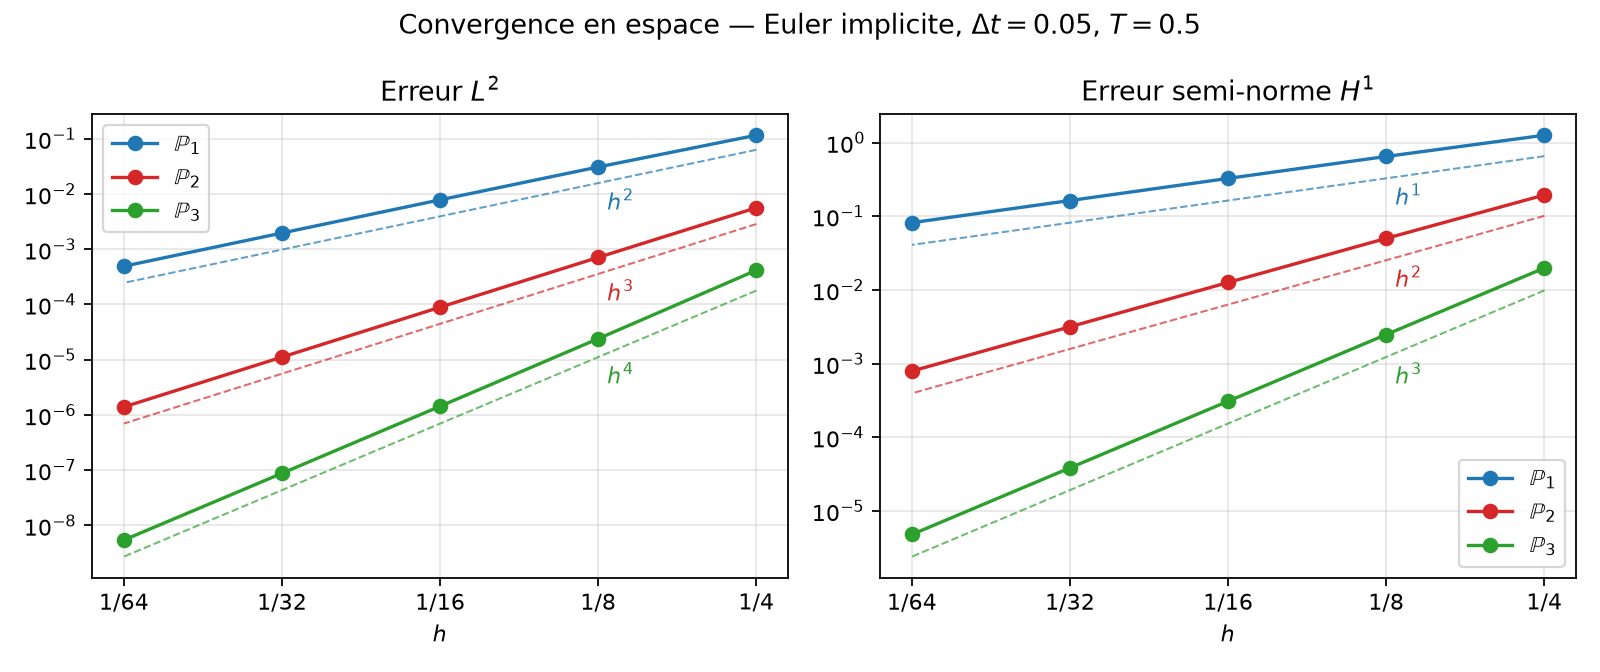
\includegraphics[width=\linewidth]{convergence_space.png}
  \caption{Convergence en espace. Les pointillés indiquent les pentes théoriques $h^{k+1}$ ($L^2$) et $h^k$ ($H^1$).}
  \label{fig:space}
\end{figure}

\begin{table}[H]
  \centering\small
  \TabSpace
  \caption{Erreurs et ordres de convergence en espace (maillages $N\times N$ de triangles, $h=1/N$).}
  \label{tab:space}
\end{table}

Les ordres observés convergent vers $k+1$ en $L^2$ et $k$ en $H^1$ pour $k=1,2,3$ :
$2{,}00 / 1{,}00$, $3{,}00 / 2{,}00$ et $4{,}01 / 3{,}00$ sur les maillages les plus fins
(tableau~\ref{tab:space}). Avec $\mathbb{P}_3$ et $N=64$, l'erreur $L^2$ atteint $5\cdot10^{-9}$.
Pour une erreur cible de $10^{-5}$, il faut environ $4\,000$ ddl en $\mathbb{P}_2$, contre bien plus de
$10^{5}$ en $\mathbb{P}_1$ (par extrapolation) : c'est l'intérêt des éléments d'ordre élevé
pour des solutions régulières.

\subsection{Isoler l'erreur temporelle}
On prend une solution non polynomiale en temps :
\begin{equation}
  u_{\text{ex}} = e^{-t}\left[\sin(\pi x)\sin(\pi y) + x + y\right], \qquad
  f = e^{-t}\left[(2\kappa\pi^2-1)\sin(\pi x)\sin(\pi y) - (x+y)\right].
\end{equation}
La condition de Dirichlet $g = e^{-t}(x+y)$ dépend alors du temps, ce qui teste aussi le lifting. Pour
rendre l'erreur spatiale négligeable, on utilise $\mathbb{P}_3$ avec $N=48$ (erreur spatiale de l'ordre
de $10^{-8}$ d'après le tableau~\ref{tab:space}), et on intègre jusqu'à $T_f=1$.

\begin{figure}[H]
  \centering
  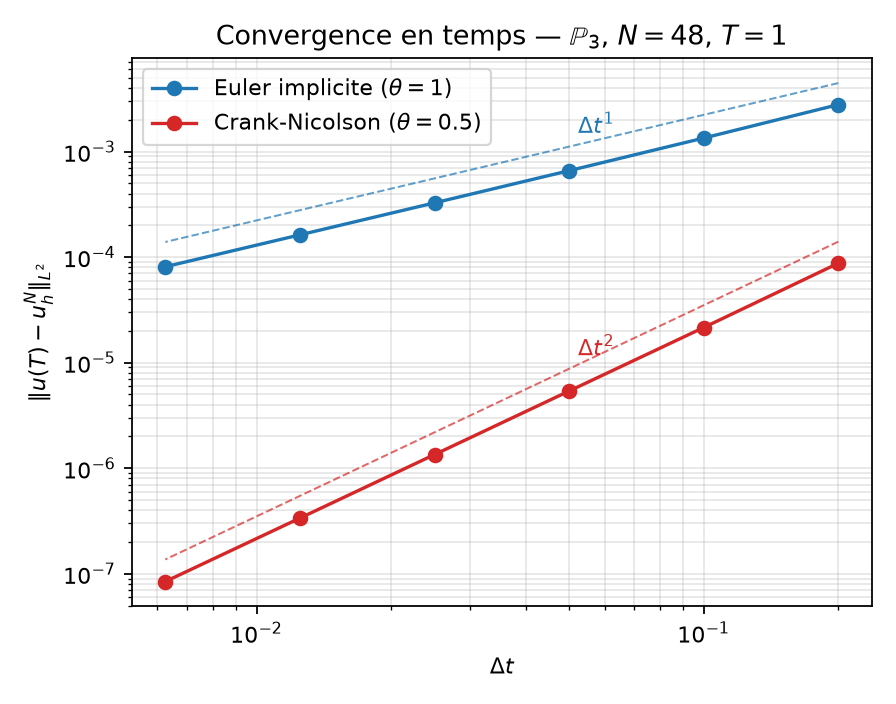
\includegraphics[width=0.62\linewidth]{convergence_time.png}
  \caption{Convergence en temps à $T_f = 1$ ($\mathbb{P}_3$, $N=48$).}
  \label{fig:time}
\end{figure}

\begin{table}[H]
  \centering\small
  \TabTime
  \caption{Erreur $L^2$ au temps final et ordres observés en temps.}
  \label{tab:time}
\end{table}

On retrouve l'ordre $1$ pour Euler implicite et l'ordre $2$ pour Crank--Nicolson
(tableau~\ref{tab:time}). À précision égale, Crank--Nicolson est très avantageux : avec
$\Delta t=0{,}2$ (5 pas), son erreur ($8{,}8\cdot10^{-5}$) est du même ordre que celle d'Euler implicite
avec $\Delta t = 0{,}00625$ (160 pas, $8{,}1\cdot10^{-5}$), soit environ 30 fois moins de pas.

%=====================================================================
\section{Stabilité : théorie et expériences}\label{sec:stab_results}
%=====================================================================
\subsection{Condition CFL d'Euler explicite}
Sur le carré unité ($\mathbb{P}_1$, $N=16$), on calcule les valeurs propres extrêmes du problème
généralisé $K\bm{w}=\lambda M\bm{w}$ restreint aux ddl intérieurs (SciPy, \texttt{eigsh}) :
\begin{gather*}
  \lambda_{\min} = \LamMin \quad\big(\text{valeur continue } 2\pi^2 = \LamMinExact\big), \\
  \lambda_{\max} = \LamMax \;\Longrightarrow\; \Delta t_c = \frac{2}{\lambda_{\max}} = \DtC .
\end{gather*}
On lance ensuite Euler explicite ($\theta=0$) sur le problème manufacturé temporel jusqu'à $T_f = 0{,}3$,
avec $\Delta t = \RatioStable\,\Delta t_c$ puis $\Delta t = \RatioUnstable\,\Delta t_c$.

\begin{figure}[H]
  \centering
  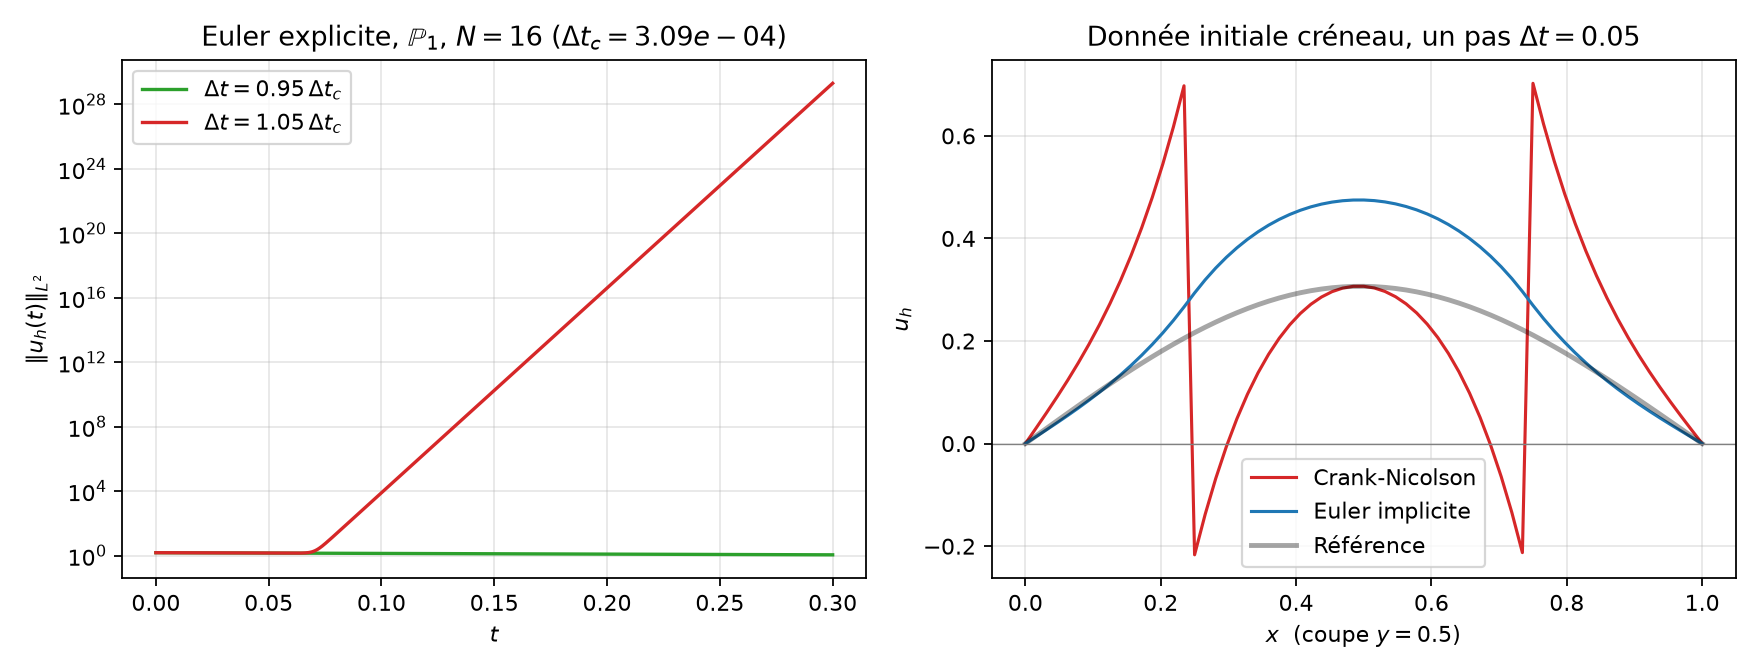
\includegraphics[width=\linewidth]{stability.png}
  \caption{Gauche : norme $L^2$ de la solution d'Euler explicite juste en dessous et juste au-dessus de
  la limite théorique. Droite : coupe $y=0{,}5$ après un pas $\Delta t = 0{,}05$ à partir d'un créneau
  ($\mathbb{P}_1$, $N=64$).}
  \label{fig:stab}
\end{figure}

Juste sous la limite, la solution reste bornée ($\|u_h(T_f)\|_{L^2} = \NormStable$). Juste au-dessus,
elle explose ($\|u_h(T_f)\|_{L^2} \approx \NormUnstable$). Le mode instable, initialement de l'ordre
de l'erreur d'arrondi, est amplifié d'un facteur $|R| = |1-\lambda_{\max}\Delta t|\approx 1{,}1$ à chaque
pas : il devient visible après environ $200$ pas, puis croît exponentiellement (droite en échelle
logarithmique). La frontière de stabilité prédite par \eqref{eq:amplif} est donc retrouvée à $5\,\%$ près.

\subsection{Défaut de L-stabilité de Crank--Nicolson}
On part d'un créneau $u_0 = \mathbf{1}_{[0.25,0.75]^2}$, avec $f=0$, $u=0$ au bord, et on fait
\emph{un seul} pas de grande taille ($\Delta t=0{,}05$, soit $\lambda_{\max}\Delta t \gg 1$).
La référence est calculée avec Euler implicite et un pas $200$ fois plus petit.
\begin{center}
\begin{tabular}{l c c}\toprule
 & $\min u_h$ & $\max u_h$ \\ \midrule
Crank--Nicolson & $\CNmin$ & $\CNmax$ \\
Euler implicite & $\BEmin$ & $\BEmax$ \\
Référence & -- & $\REFmax$ \\ \bottomrule
\end{tabular}
\end{center}
Crank--Nicolson produit des oscillations parasites et des températures \emph{négatives}, ce qui viole
le principe du maximum : c'est l'effet de $R(z)\to-1$. Euler implicite, L-stable, amortit les
hautes fréquences et reste positif, mais il est trop diffusif à ce grand pas : son pic vaut $\BEmax$
au lieu de $\REFmax$. En pratique, on combine les deux (\emph{démarrage de Rannacher} : quelques pas
d'Euler implicite puis Crank--Nicolson), ou on choisit $\theta$ légèrement supérieur à $\frac12$.

%=====================================================================
\section{Application : plaque d'acier chauffée par un laser mobile}\label{sec:laser}
%=====================================================================
\subsection{Modèle physique}
On considère une plaque d'acier mince de dimensions $L_x\times L_y = 100\times50$~mm et d'épaisseur
$e=2$~mm, balayée par un faisceau laser gaussien. Comme $e$ est petite devant la longueur de diffusion
$\sqrt{\alpha t_{\text{on}}}\approx 14$~mm, on suppose la température uniforme dans l'épaisseur.
En intégrant l'équation de la chaleur 3D sur l'épaisseur, la convection des deux faces devient un terme
volumique :
\begin{equation}\label{eq:plate}
  \rho c\, e\, \frac{\partial T}{\partial t} - \divg(k e \nabla T) + 2h\,(T-T_a) = q_s(\bm{x},t),
  \qquad -k\nabla T\cdot\bm{n} = h\,(T-T_a) \ \text{sur } \partial\Omega,
\end{equation}
avec la densité surfacique de puissance absorbée
\begin{equation}
  q_s(\bm{x},t) = \mathbf{1}_{t\le t_{\text{on}}}\;\frac{\eta P}{2\pi s^2}
  \exp\!\left(-\frac{|\bm{x}-\bm{x}_s(t)|^2}{2s^2}\right), \qquad
  \bm{x}_s(t) = \left(x_0 + v\,t,\ L_y/2\right).
\end{equation}
En divisant par $\rho c e$, on retrouve exactement la forme \eqref{eq:strong} avec
\[
  \kappa = \alpha = \frac{k}{\rho c}, \qquad \beta = \frac{2h}{\rho c\,e}, \qquad
  h_c = \frac{h}{\rho c}, \qquad f = \frac{q_s}{\rho c\, e}, \qquad \Gamma_R = \partial\Omega .
\]

\begin{table}[H]
\centering\small
\begin{tabular}{l c r}\toprule
Paramètre & Symbole & Valeur \\ \midrule
Conductivité / masse volumique / capacité & $k,\ \rho,\ c$ & \SI{45}{W.m^{-1}.K^{-1}}, \SI{7850}{kg.m^{-3}}, \SI{460}{J.kg^{-1}.K^{-1}} \\
Diffusivité & $\alpha$ & \SI{1.246e-5}{m^2.s^{-1}} \\
Coefficient de convection, ambiante & $h,\ T_a$ & \SI{25}{W.m^{-2}.K^{-1}}, \SI{20}{\celsius} \\
Puissance, absorptivité, rayon & $P,\ \eta,\ s$ & \SI{400}{W}, $0{,}5$, \SI{1.5}{mm} \\
Départ, vitesse, durée de chauffe & $x_0,\ v,\ t_{\text{on}}$ & \SI{20}{mm}, \SI{4}{mm.s^{-1}}, \SI{15}{s} \\
Durée simulée & $T_f$ & \SI{25}{s} \\ \bottomrule
\end{tabular}
\caption{Paramètres du cas laser.}
\end{table}

Le nombre de Péclet de la source, $\mathrm{Pe} = v s/\alpha \approx 0{,}48$, est modéré : la diffusion
domine encore à l'échelle du spot, d'où des isothermes en forme de comète peu allongée.

\textbf{Discrétisation.} Maillage de $200\times100$ rectangles coupés en triangles ($h=0{,}5$~mm, soit
3 éléments par rayon $s$), $\mathbb{P}_1$ (\LaserNdofs\ ddl), Crank--Nicolson avec $\Delta t = 0{,}05$~s
(500 pas), solveur LU. Le calcul séquentiel prend \LaserWall~s, post-traitement compris.

\subsection{Résultats}
\begin{figure}[H]
  \centering
  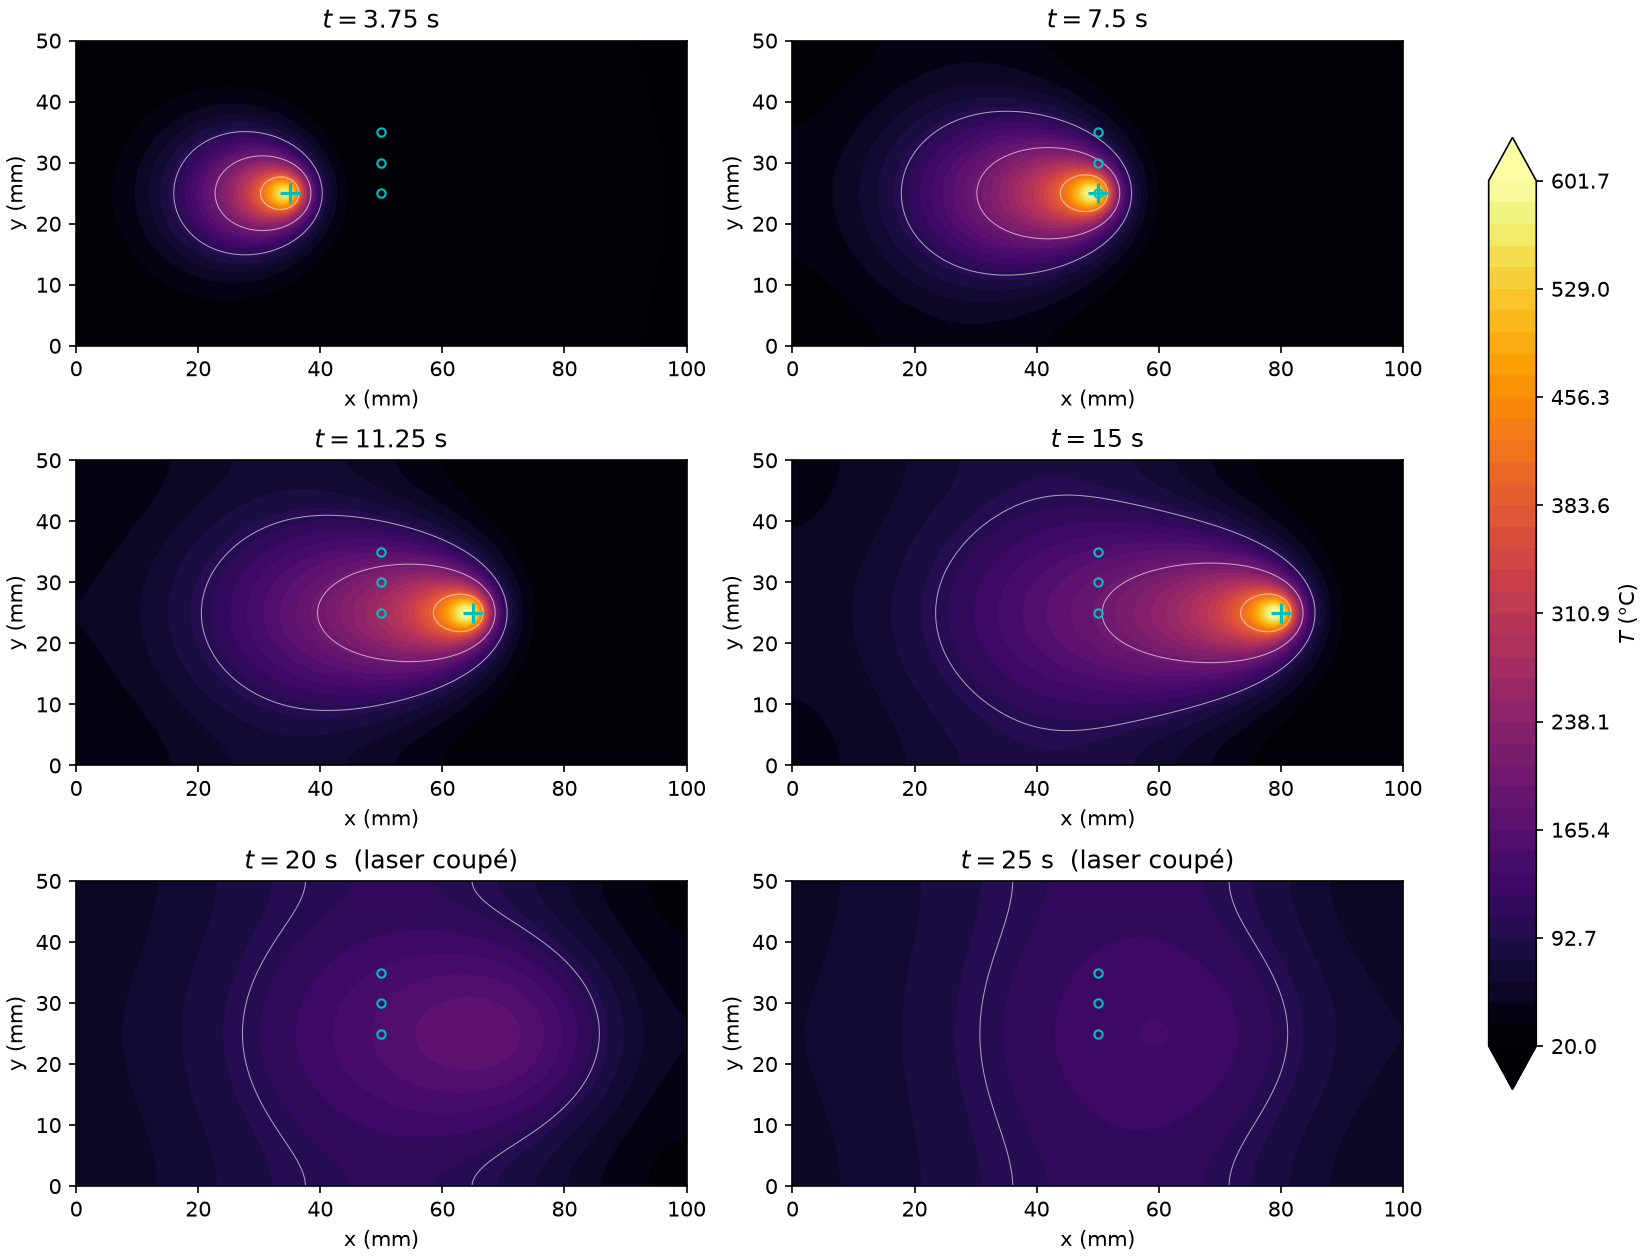
\includegraphics[width=\linewidth]{laser_snapshots.png}
  \caption{Champ de température. La croix marque le centre du spot laser et les cercles les trois sondes
  ($x=50$~mm, à $0$, $5$ et $10$~mm de la trajectoire). Isothermes blanches : 100, 200, 400 et \SI{600}{\celsius}.}
  \label{fig:snap}
\end{figure}

\begin{figure}[H]
  \centering
  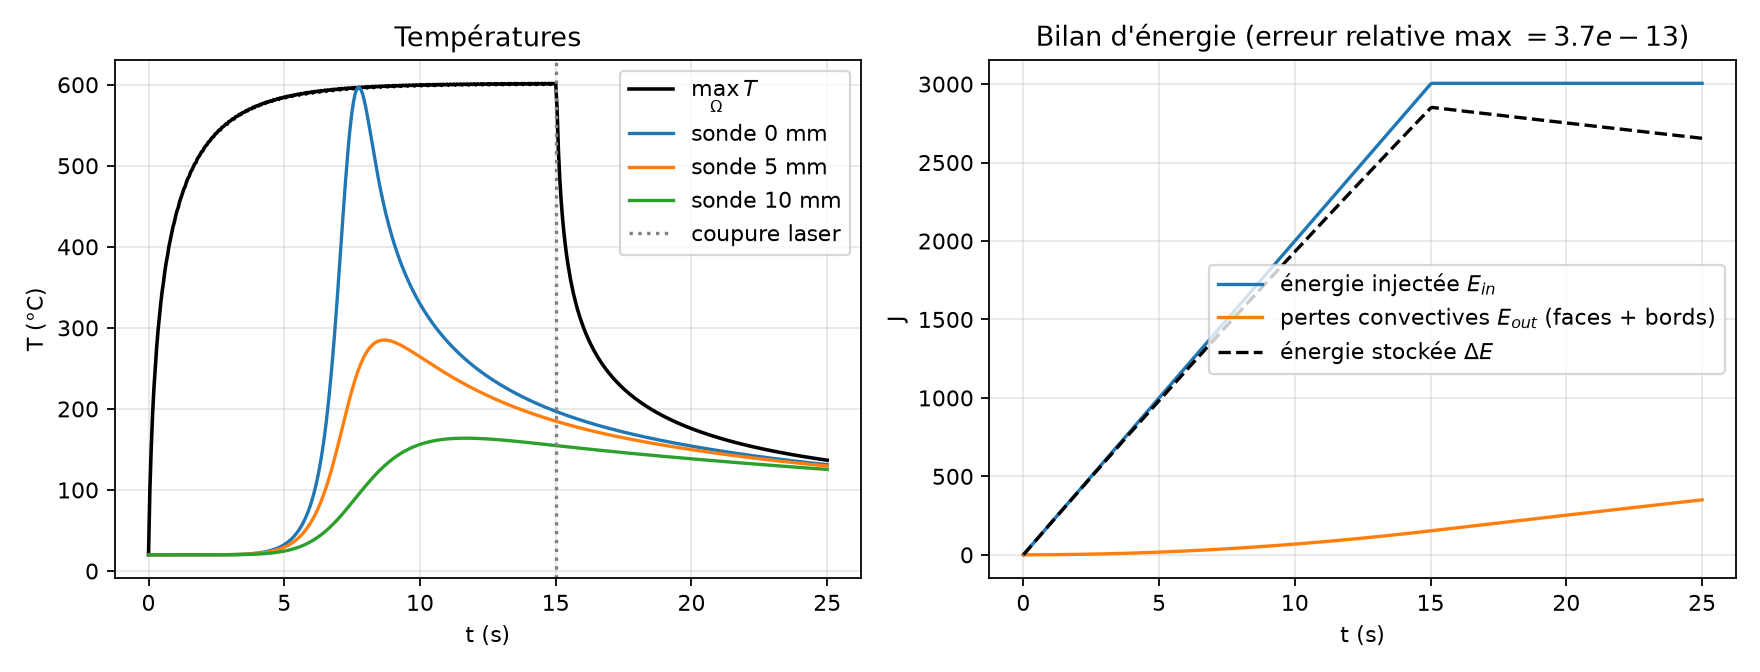
\includegraphics[width=\linewidth]{laser_history.png}
  \caption{Gauche : évolution du maximum de température et des sondes. Droite : bilan d'énergie.}
  \label{fig:hist}
\end{figure}

La figure~\ref{fig:hist} montre que la température maximale s'établit en quelques secondes à un
régime quasi stationnaire dans le repère de la source. Elle atteint \LaserTmax~\si{\celsius} à la
coupure, puis chute brutalement après $t_{\text{on}}$. Les sondes enregistrent des pics de
\LaserProbeA, \LaserProbeB\ et \LaserProbeC~\si{\celsius} à $0$, $5$ et $10$~mm de la trajectoire. Plus
on s'éloigne de la trajectoire, plus le pic est faible et tardif, ce qui traduit le temps de diffusion
latérale. Après la coupure, la plaque s'homogénéise lentement : le temps caractéristique de
refroidissement par les faces est $\rho c e/(2h)\approx\SI{144}{s}$, bien plus long que la durée simulée.

\subsection{Contrôles de qualité}
\paragraph{Conservation de l'énergie.} On accumule au cours du calcul l'énergie injectée $E_{in}$, les
pertes $E_{out}$ (faces et bords) et la variation d'énergie stockée $\Delta E = \rho c e\int_\Omega (T-T_0)\dd x$,
avec les mêmes moyennes en $\theta$ que le schéma. L'identité discrète $\Delta E = E_{in}-E_{out}$
(section~\ref{sec:energy}) est vérifiée avec une erreur relative maximale de $\LaserBalance$, soit la
précision machine. On obtient $E_{in} = \LaserEin$~J, $E_{out}=\LaserEout$~J (\LaserLossPct~\% de
l'apport) et $\Delta E = \LaserEstored$~J.

Deux subtilités sont apparues pendant le développement :
\begin{itemize}
  \item La valeur théorique de l'apport est $\eta P\, t_{\text{on}} = 3000$~J. L'écart de $5$~J vient du
        pas qui contient la coupure : Crank--Nicolson y moyenne $f^{n}$ (laser allumé) et $f^{n+1}$
        (laser éteint), ce qui ajoute exactement $\frac12\Delta t\,\eta P = 5$~J. Ce n'est pas une
        erreur de conservation, mais la discrétisation d'une source discontinue en temps. Cet écart tend
        vers $0$ avec $\Delta t$.
  \item Sur un maillage grossier ($h > s$), le bilan n'était d'abord vérifié qu'à $10^{-5}$ près. La cause :
        $\int_\Omega f\dd x$ était intégré avec un degré de quadrature plus faible que le second membre
        $\int_\Omega f v_h\dd x$ du solveur. En calculant l'apport comme $\int_\Omega f\cdot 1_h\dd x$
        avec $1_h\in V_h$, on utilise la même quadrature, et l'identité redevient exacte.
\end{itemize}

\paragraph{Indépendance au maillage et au pas de temps.}
\begin{table}[H]
  \centering\small
  \TabLaserConv
  \caption{Sensibilité du pic de température aux paramètres de discrétisation (référence : $h=0{,}25$~mm, $\Delta t = 0{,}05$~s).}
  \label{tab:laserconv}
\end{table}
Le pic converge avec le raffinement : l'écart passe de $1{,}2$~\si{\celsius} entre $h=1$ et
$h=0{,}5$~mm à $0{,}3$~\si{\celsius} entre $h=0{,}5$ et $h=0{,}25$~mm, soit un rapport d'environ 4,
cohérent avec la convergence d'ordre 2 de $\mathbb{P}_1$ pour une quantité ponctuelle régulière. Le
pas de temps a un effet encore plus faible sur $\max T$ (environ $0{,}06$~\si{\celsius} entre
$\Delta t = 0{,}1$ et $0{,}025$~s). La sonde sur la trajectoire est plus sensible à $\Delta t$
($0{,}9$~\si{\celsius} à $\Delta t=0{,}1$~s), car son pic est très bref et n'est échantillonné qu'aux
instants $t^n$. Le maillage $h=0{,}5$~mm est donc précis à environ $0{,}05\,\%$ près sur le pic.

\subsection{Scalabilité forte sur un CPU hybride}\label{sec:scaling}
\paragraph{Protocole.} L'étude est faite sur la machine de l'auteur, un portable équipé d'un
\ScalCPU. Ce processeur est \emph{hybride} : 4 cœurs performants (P-cores, avec hyperthreading)
et 4 cœurs efficaces (E-cores, plus lents), soit 8 cœurs physiques et 12 threads. Le cas laser est
résolu sur un maillage $600\times300$ (\ScalNdofs\ ddl, 500 pas de temps) avec CG + BoomerAMG, sur
$p = 1, 2, 4, 8$ processus MPI. Chaque configuration est lancée \ScalReps\ fois et on garde le temps
médian. Pour des mesures fiables, chaque processus est fixé sur un cœur (\texttt{-bind-to core}) et
limité à un seul thread (\texttt{OMP\_NUM\_THREADS=1}). Script : \texttt{scripts/study\_scaling.py}.

On note $T_p$ le temps avec $p$ processus, l'accélération $S(p) = T_1/T_p$ et l'efficacité
$E(p) = S(p)/p$.

\begin{table}[H]
  \centering\small
  \TabScaling
  \caption{Scalabilité forte du cas laser (\ScalNdofs\ ddl, CG + BoomerAMG). Dispersion : écart
  relatif entre le plus lent et le plus rapide des \ScalReps\ lancements.}
  \label{tab:scaling}
\end{table}
\begin{figure}[H]
  \centering
  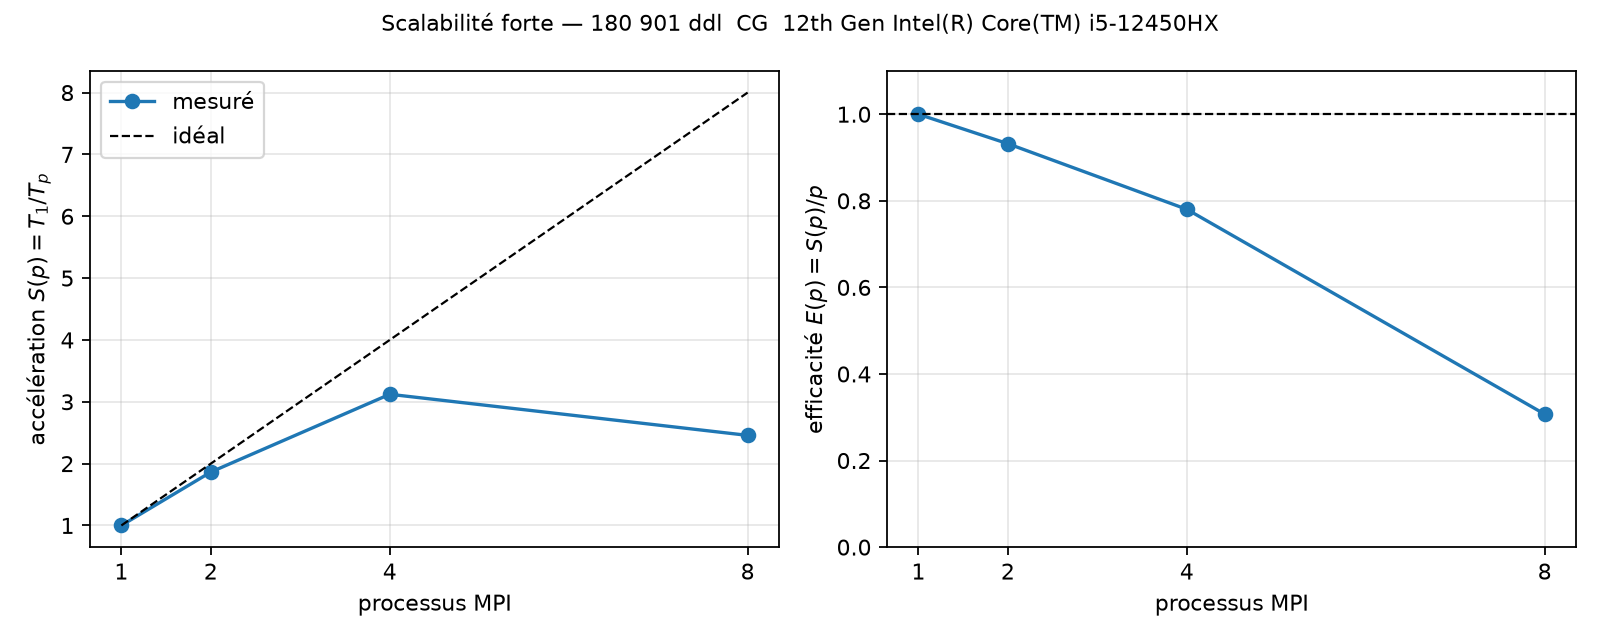
\includegraphics[width=\linewidth]{scaling.png}
  \caption{Accélération et efficacité parallèle mesurées.}
  \label{fig:scaling}
\end{figure}

\paragraph{Résultats.} Les mesures sont très reproductibles : au plus \ScalMaxSpread~\% d'écart entre
lancements. Le pic de température est identique pour tous les lancements à $\ScalTmaxSpread$~\si{\celsius}
près, quel que soit $p$, ce qui confirme que la partition ne change pas le résultat. L'accélération
est presque idéale à 2 processus ($S=\ScalSTwo$, $E=\ScalETwo~\%$) et encore bonne à 4
($S=\ScalSFour$, $E=\ScalEFour~\%$). En revanche, à 8 processus le calcul est \emph{plus lent} qu'à 4
($T_8 = \ScalTEight$~s contre $T_4=\ScalTFour$~s), et l'efficacité tombe à $\ScalEEight~\%$.

\paragraph{Interprétation.} Trois effets peuvent expliquer ce comportement :
\begin{itemize}
  \item \textbf{Déséquilibre de charge sur un CPU hybride.} DOLFINx partitionne le maillage en
        morceaux de même taille, comme si tous les cœurs étaient identiques. Or CG est
        \emph{synchrone} : à chaque itération, les produits scalaires demandent une réduction
        globale (\texttt{MPI\_Allreduce}), et tous les processus attendent le plus lent. Jusqu'à 4
        processus, l'ordonnanceur peut tout placer sur les P-cores. À 8, la moitié des processus
        tourne sur les E-cores, plus lents, et ce sont eux qui imposent le rythme.
  \item \textbf{Bande passante mémoire.} Le produit matrice--vecteur creux et les opérations de
        l'AMG sont limités par la mémoire, pas par le calcul. Tous les cœurs partagent les mêmes
        canaux mémoire, et ajouter des processus n'augmente plus le débit une fois ces canaux
        saturés. C'est sans doute pour cela que l'efficacité est déjà de $\ScalEFour~\%$ à 4.
  \item \textbf{Solveur et partie séquentielle.} Le nombre d'itérations de CG passe de $5{,}97$ à
        $6{,}81$ par pas à 8 processus ($+14\,\%$), car l'AMG parallèle construit une hiérarchie
        moins efficace sur une partition plus fine. S'y ajoutent les parties qui ne se parallélisent
        pas (boucle Python, post-traitement), qui limitent l'accélération selon la loi d'Amdahl.
\end{itemize}
Ces trois effets sont des hypothèses compatibles avec les mesures, pas des faits démontrés. Pour les
séparer, il faudrait refaire l'étude avec 4 processus fixés sur les E-cores puis sur les P-cores
(effet de l'hybride), mesurer le débit mémoire avec STREAM (effet de la bande passante), et profiler
le temps passé dans le solveur et dans Python (loi d'Amdahl).

\paragraph{Leçons pratiques.} Sur ce portable, 4 processus est le bon choix. Pendant le développement,
une première version du post-traitement recompilait les formes UFL à chaque pas : elle était même
plus lente à 2 processus qu'à 1. Précompiler ces formes hors de la boucle en temps a été
indispensable pour obtenir une accélération. Sur un vrai cluster aux cœurs homogènes et avec plus de
bande passante par nœud, on s'attend à une bien meilleure scalabilité. C'est la prochaine étape
naturelle (\texttt{sbatch} avec SLURM).

%=====================================================================
\section{Limites et perspectives}
%=====================================================================
\begin{itemize}
  \item \textbf{Non-linéarités} : $k(T)$ et $c(T)$ dépendent fortement de la température dans l'acier.
        Le problème devient non linéaire (\texttt{NonlinearProblem}, méthode de Newton) et la matrice
        doit être réassemblée à chaque pas.
  \item \textbf{Rayonnement} : à $\SI{600}{\celsius}$, les pertes radiatives
        $\varepsilon\sigma(T^4-T_a^4)$ dominent la convection naturelle. Le modèle actuel sous-estime
        donc les pertes.
  \item \textbf{Modèle 3D} pour une plaque épaisse ou un apport localisé en surface (gradient dans
        l'épaisseur), avec maillage Gmsh raffiné près de la trajectoire.
  \item \textbf{Adaptativité} : pas de temps adaptatif (estimateur basé sur la différence entre Euler
        implicite et Crank--Nicolson) et raffinement de maillage qui suit la source.
  \item \textbf{Performance HPC} : refaire l'étude de scalabilité forte sur un cluster aux cœurs
        homogènes, ajouter une étude de scalabilité faible, partitionner en tenant compte de la vitesse
        des cœurs sur un CPU hybride, et comparer LU et CG--AMG en 3D.
\end{itemize}

%=====================================================================
\section{Conclusion}
%=====================================================================
On a développé avec FEniCSx un solveur éléments finis générique pour l'équation de la chaleur
instationnaire, avec conditions de Dirichlet, Neumann et Robin, échange volumique et $\theta$-schéma. Le
code est \emph{vérifié} : tous les ordres de convergence théoriques en espace ($\mathbb{P}_1$ à
$\mathbb{P}_3$) et en temps (ordres 1 et 2) sont retrouvés. Les propriétés de stabilité prédites par
l'analyse du facteur d'amplification (limite CFL d'Euler explicite, défaut de L-stabilité de
Crank--Nicolson) sont reproduites quantitativement. Le cas applicatif de la source laser mobile est
accompagné de contrôles de qualité : conservation discrète de l'énergie à la précision machine,
indépendance au maillage et au pas de temps, résultats parallèles identiques aux résultats séquentiels.
L'étude de scalabilité forte montre une bonne accélération jusqu'à 4 processus ($S = \ScalSFour$) et
met en évidence les limites d'un CPU hybride au-delà.

\begin{thebibliography}{9}
\bibitem{thomee} V.~Thomée, \emph{Galerkin Finite Element Methods for Parabolic Problems}, 2\textsuperscript{e} éd., Springer, 2006.
\bibitem{ern} A.~Ern, J.-L.~Guermond, \emph{Theory and Practice of Finite Elements}, Springer, 2004.
\bibitem{dolfinx} I.~A.~Baratta et al., \emph{DOLFINx: the next generation FEniCS problem solving environment}, Zenodo, 2023. \url{https://doi.org/10.5281/zenodo.10447666}
\bibitem{roache} P.~J.~Roache, \emph{Code verification by the method of manufactured solutions}, J.~Fluids Eng.~124(1), 2002.
\bibitem{rannacher} R.~Rannacher, \emph{Finite element solution of diffusion problems with irregular data}, Numer.~Math.~43, 1984.
\end{thebibliography}

\appendix
\section{Reproduction des résultats}\label{app:repro}
\begin{lstlisting}[language=bash]
# Environnement (conda-forge)
conda env create -f environment.yml && conda activate fenicsx-heat
# Toutes les études + figures (~10 min sur 2 coeurs)
./run_all.sh
# Exécution parallèle du cas laser et étude de scalabilité forte
cd scripts && mpirun -n 4 python laser.py --nx 400 --solver cg
python study_scaling.py --nx 600 --np 1 2 4 8 --reps 3
# Régénérer les tableaux et compiler le rapport
cd ../report && python make_tables.py && latexmk -pdf rapport.tex
\end{lstlisting}
Le champ de température est exporté au format XDMF (\texttt{results/laser.xdmf}) et peut être ouvert
dans ParaView pour l'animer.

\end{document}
